\documentclass[conference]{IEEEtran}
\usepackage[T1]{fontenc}
\usepackage{amsmath,amssymb,booktabs,graphicx,array,microtype,url}
\usepackage[hidelinks]{hyperref}
\graphicspath{{figures/}{figures/generated/}}
\setlength{\textfloatsep}{12pt plus 2pt minus 2pt}
\setlength{\dbltextfloatsep}{12pt plus 2pt minus 2pt}
\newcommand{\code}[1]{\texttt{#1}}
\newcommand{\CoreCaseCount}{42}
\newcommand{\CoreKeyCount}{4,520}
\newcommand{\CoreMacCount}{13,557,824}
\newcommand{\FpCaseCount}{130,009}
\newcommand{\TensorBytes}{5,707,008}
\newcommand{\OraclePairCount}{99,244}
\newcommand{\RationalCaseCount}{5,010}
\newcommand{\TieDifference}{16}
\newcommand{\BfRelative}{0.00395188}
\newcommand{\BfAbsolute}{0.0328097}

\title{FP4 Sparse Indexing on a Unified\newline CPU/GPU/NPU--UCIe Memory System}
\author{\IEEEauthorblockN{Anonymous Artifact Authors}\IEEEauthorblockA{Digital hardware design and reproducibility study}}
\begin{document}
\maketitle
\begin{abstract}
Learned sparse-attention indexing combines low-precision arithmetic, selection, and data movement. We implement a post-projection CSA2 indexer as synthesizable digital hardware connected to CPU/Vortex/CoralNPU through native 256-bit AXI, AXI2Flit, UCIe, and one online memory simulator. A 16-lane E2M1 FP4 datapath with E8M0 group scales computes signed weighted-ReLU scores across 32 heads. One shared key buffer, a stable Top-512 heap, an explicit FP32 rounding contract, and a DMA endpoint support full scan, candidate-only scan, and committed-index reuse. Completion depends on actual memory responses. Native H32/N640/K512 FULL and REUSE require 670,572 and 115,776 busy cycles, respectively; every selected record and 147,456 gathered bytes are verified per command. The mapped core has 0.301 mm$^2$ of cell area in a 28-nm HPC+ library at TT 0.9V 25C. It meets the nominal 2-ns timing target with ideal clocking and only 6 fs reported setup slack.
 Validation includes \CoreCaseCount{} core cases, \FpCaseCount{} floating-point cases, learned-weight operator fixtures, and AXI fault/backpressure checks. Projection, candidate-block generation, final attention, full-model quality, and SRAM-CIM physical implementation remain outside the demonstrated scope.
\end{abstract}
\begin{IEEEkeywords}
Digital IC, sparse attention, FP4, near-memory computing, RTL, AXI, UCIe
\end{IEEEkeywords}

\section{Introduction}
The engineering value of a sparse-attention gate depends on more than an algorithm name or a stand-alone score kernel. Input records must reach the hardware, arithmetic must preserve a specified selection contract, selected data must be fetched, and completion must return through the processor's actual memory path. A replay-only timeline cannot establish those dependencies.

CSA2, released with DeepSeek-V4.1-Flash in September 2026, provides a current target with published model configuration, low-precision formats, and reference code~\cite{csa2,csa2code}. It develops the learned weighted-ReLU indexing approach associated with DSA~\cite{dsa}, with compressed representations and cross-layer KV/index reuse. These algorithmic mechanisms belong to the cited work. Our contribution is a bounded digital implementation and its integration evidence.

The starting system is the fixed StorageStacked revision identified in the artifact~\cite{upstream}. It retains three processing sources and its online return path. CPU execution uses gem5's timing CPU, Vortex uses SimX, and CoralNPU uses its RTL-based model. This is an SE system, with CPU program/stack memory outside the remote target. It is not a full-chip RTL model or a coherent three-device memory system.

We make three concrete engineering contributions. First, a complete FP4 score-to-selection datapath replaces fixed-size pooled-block gating with 32-head, 128-dimensional indexing and K up to 512. Second, a memory-side register/DMA endpoint makes ordinary traffic, candidate reads, result writes, and selected-KV copies share the existing memory authority and time axis. Third, frozen official-source slices, an independent numerical oracle, backpressure/error checks, and bounded synthesis evidence connect the algorithm contract to the actual RTL. None implies a new sparse-attention algorithm or an unmeasured full-model speedup.

\begin{figure*}[t]
\centering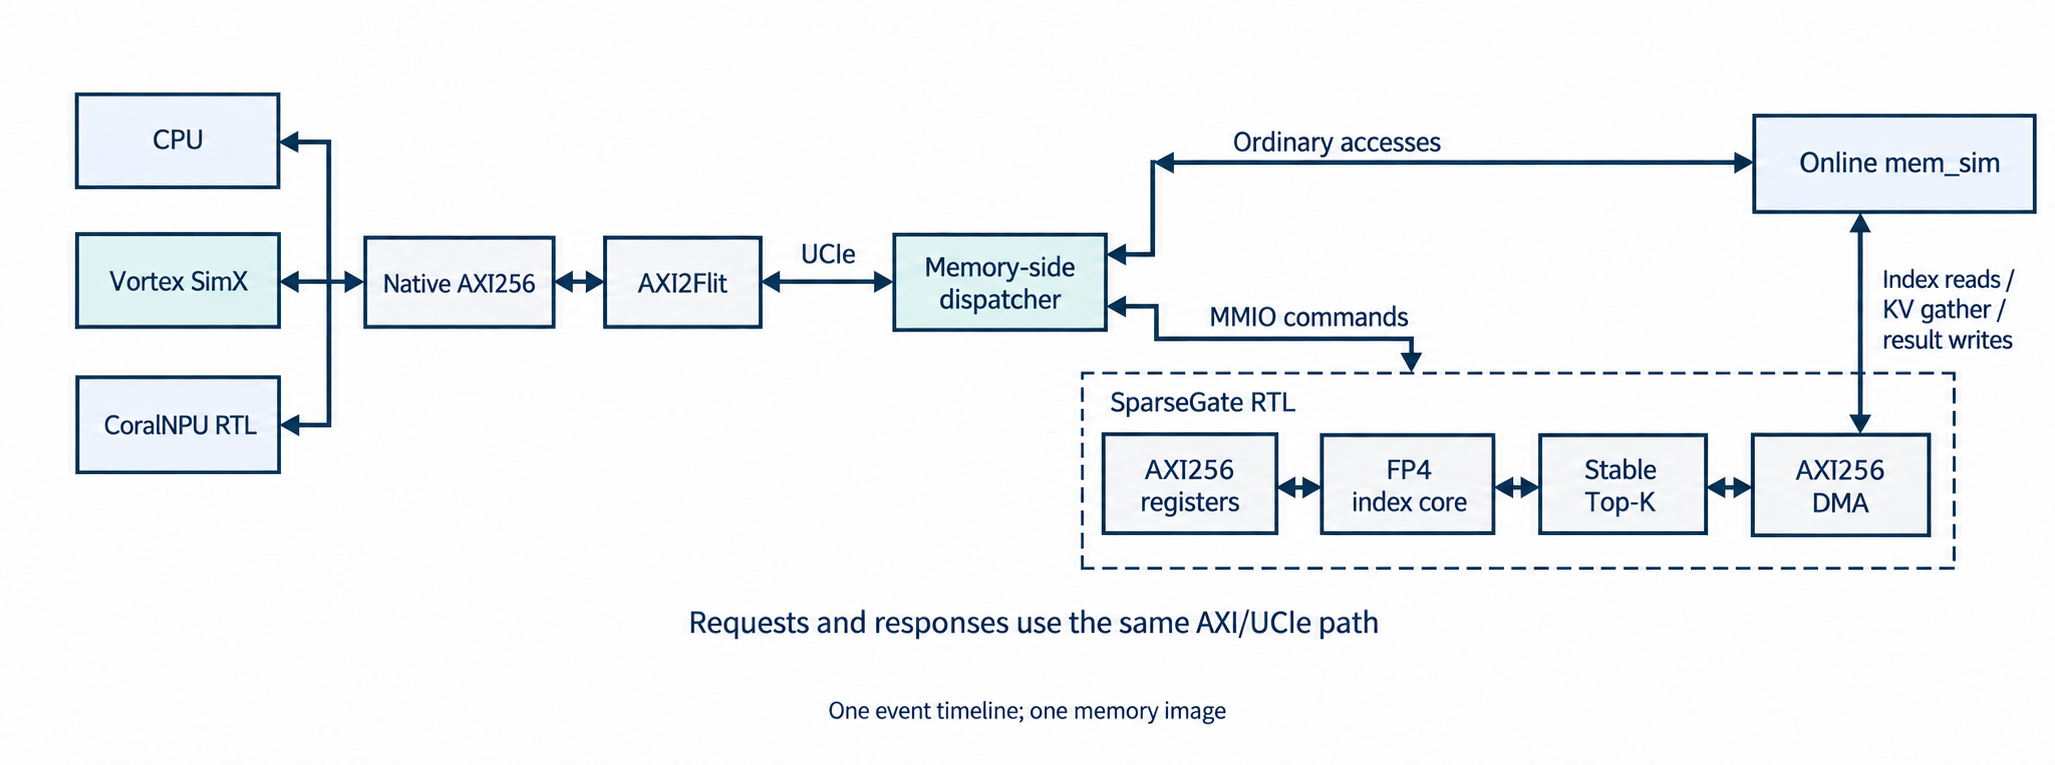
\includegraphics[width=\textwidth]{system.png}
\caption{System placement. SparseGate is after UCIe; ordinary accesses retain a bypass. The C++ memory-side dispatcher is a verification adapter, while the register endpoint, score/selection core, and DMA are synthesizable RTL. Return data and completion follow the original protocol path. Conceptual illustration; exact protocol contracts are in the artifact.}
\label{fig:system}
\end{figure*}

\section{From Pooled Gating to Learned Indexing}
\subsection{What the thesis provides}
Wang's thesis~\cite{wang} describes a substantial pooled-gating architecture: 128 Blocks, 32 Cells per Block, 32-value BF16 storage per Cell, mean pooling, spatial reduction, and 32 independent Top-K modules. Its stated mapping uses 32 blocks of tokens and selects 12. The fourfold GQA replication yields 256 KiB of Kmean payload for 64 KiB of distinct summaries. These capacities are arithmetic deductions from the thesis, not measurements of our design.

The thesis's bitwise competition is a combinational chain within a clock cycle: it selects one winner per cycle, rather than consuming one clock per score bit. Expanding that network directly to long token sequences and Top-512 is not the implemented architecture here. The thesis also treats the SRAM-CIM cell as a black box for digital synthesis and obtains macro estimates from cited work. Its reported 7-nm values involve normalization from 28-nm results. We neither reuse those values nor claim a new physical SRAM-CIM macro. Author-delivered RTL and macro characterization were unavailable; this work rearchitects from the documented design concepts.

\subsection{Target operator and scope}
For one query, the post-projection score is
\begin{equation}
 s_i=\sum_{h=0}^{H-1}w_h\operatorname{ReLU}\!\left(\sum_{d=0}^{127}q_{h,d}k_{i,d}\right),\quad H\le32.
\label{eq:score}
\end{equation}
The same index key $k_i$ serves all heads. The input BF16 $w_h$ already includes the official projected head weight and its $D^{-1/2}H^{-1/2}$ scale; the RTL does not apply that normalization again. The learned $w_h$ may be negative. ReLU therefore occurs after each complete head dot product and before the signed weighting; moving it across the head sum changes the algorithm. We perform no early pruning based on a false nonnegative-contribution assumption.

The official CSA2 configuration uses 32 index heads, dimension 128, and Top-512. Here $N$ counts compressed index/KV records and $i$ is their raw position, not an original-token identifier. Software applies the official offset when combining compressed indices with sliding-window entries and handles invisible-entry $-1$ placeholders. Its candidate-source layer builds a block pool with width eight and up to 2048 blocks; a latest partial block is retained. Our hardware consumes an expanded, ascending unique list of valid candidate indices. Block-pool production, compression, Q/K projections, RMSNorm, RoPE, quantization, and sparse attention stay in the processor/software boundary. For prefill, software intersects the block mask with visible positions before issuing physical reads. The hardware modes described below are execution modes of this operator boundary, not a claim to implement every CSA2 layer role.

\section{Numeric and Microarchitectural Design}
\subsection{Packed records and exact group arithmetic}
Indexer values use E2M1 FP4 and one E8M0 scale per 32 dimensions~\cite{csa2code,mx}. FP4 is not a signed uniform INT4 format. Doubling an E2M1 value gives the integer set
\begin{equation}
 \mathcal M=\{0,\pm1,\pm2,\pm3,\pm4,\pm6,\pm8,\pm12\}.
\end{equation}
A group dot $D_{h,g}=\sum_{j=0}^{31}m^q_{h,g,j}m^k_{i,g,j}$ is exact in the range $[-4608,4608]$. For scale bytes $e_q,e_k$, its FP32 contribution is
\begin{equation}
 a_{h,g}=\operatorname{RNE}_{32}\!\left(D_{h,g}\,2^{e_q+e_k-256}\right).
\end{equation}
The implementation adds the four groups in order, applies ReLU, multiplies by a finite signed BF16 weight expanded exactly to FP32, and adds heads in order. Each floating-point operation uses round-to-nearest-even with gradual underflow. For fetched records, E8M0 byte 255, nonfinite weights, and intermediate FP32 overflow cause an error with no successful selection output. Unread keys in candidate-only mode are not format-checked.

This explicit contract supports bit-exact RTL/oracle comparison. It does not promise bit-exact equivalence to a GPU kernel with a different accumulation order or BF16 output rounding. Ties are ordered by smaller index, including equivalence of positive and negative zero.

\begin{figure*}[t]
\centering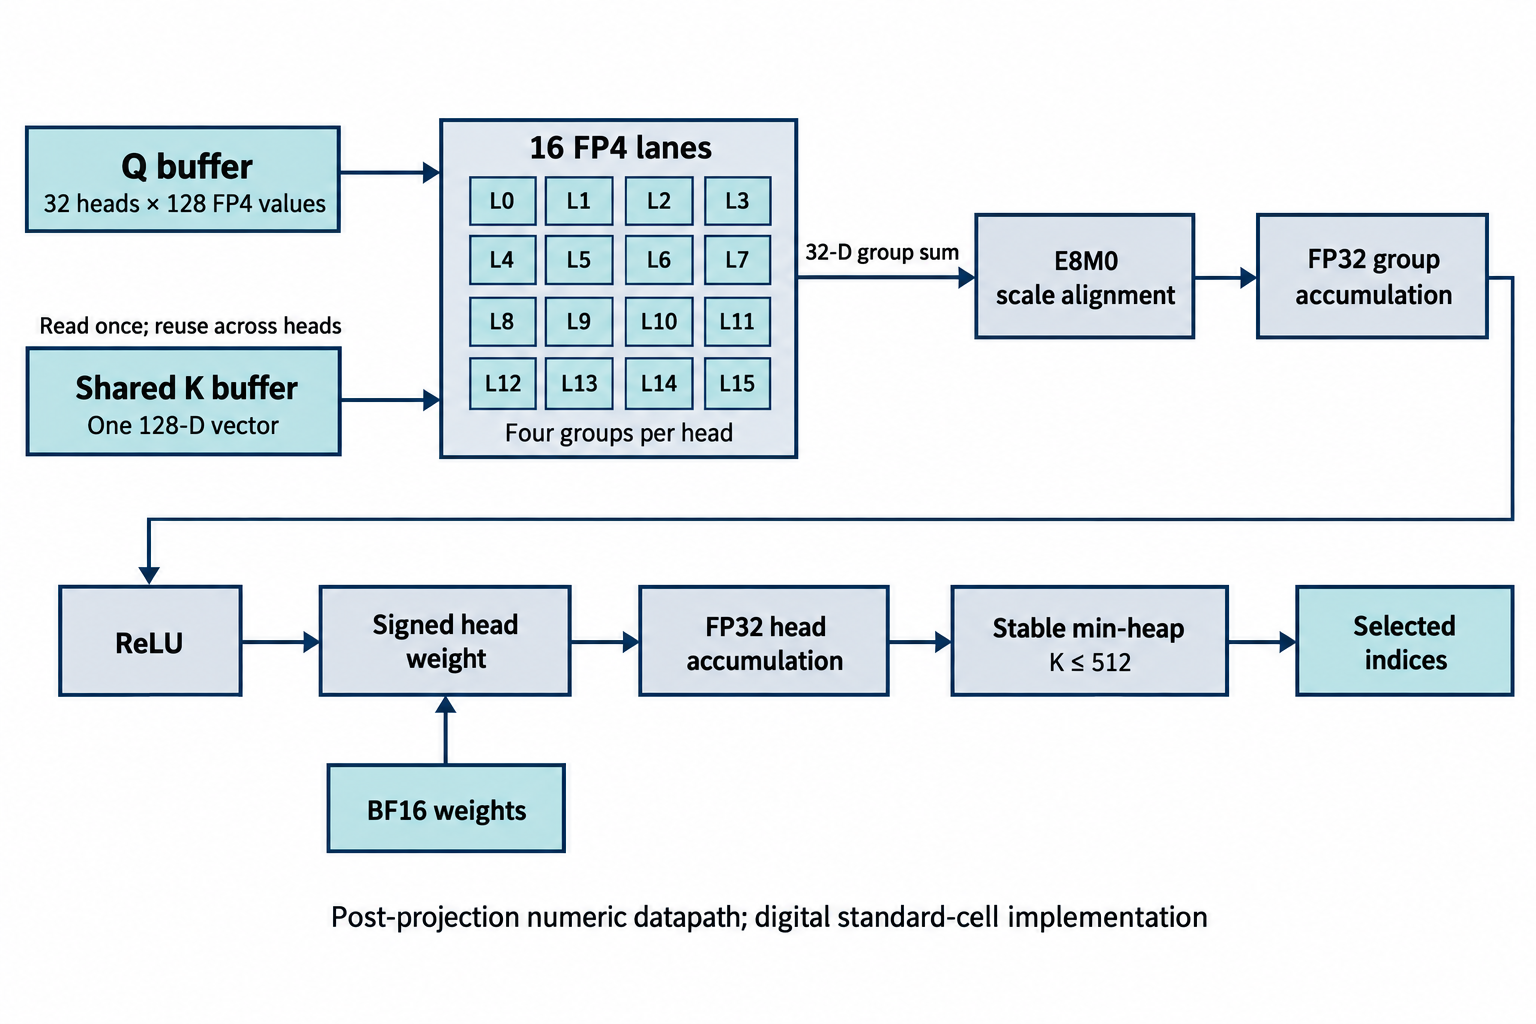
\includegraphics[width=.95\textwidth]{core.png}
\caption{Actual arithmetic organization. The baseline has 16 FP4 lanes. A group needs two lane batches before FP32 scale conversion and accumulation. Four groups form a head dot; ReLU, signed weighting, and head reduction precede heap insertion. Storage arrays have no physical SRAM-macro binding.}
\label{fig:core}
\end{figure*}

\subsection{Shared key buffer and bounded selection}
The Q buffer holds 32 records, each containing 64 B packed values, four scale bytes, and a two-byte weight: 2240 B of logical payload. One 68-B key buffer is reused for all heads. Each physical Q or K record occupies 96 B, or three aligned AXI256 beats. Padding is counted as traffic. The design reads each scored key record once instead of creating one memory copy per index head.

A min-heap holds at most 512 pairs of a 32-bit score and a 32-bit index, for 4 KiB of logical payload. The root is the worst retained candidate under the stable ordering. An arriving score either appends, replaces the root, or is rejected; heap repair takes $O(\log K)$ comparisons with at most two children considered per step. The core has bounded valid/ready result and score interfaces. The wrapper collects the heap output into a separate 4-KiB result cache and insertion-sorts it by index for positional output. This simple $O(K^2)$ worst-case positional sort is an explicit area/latency tradeoff, not hidden constant-time sorting.

\begin{figure*}[t]
\centering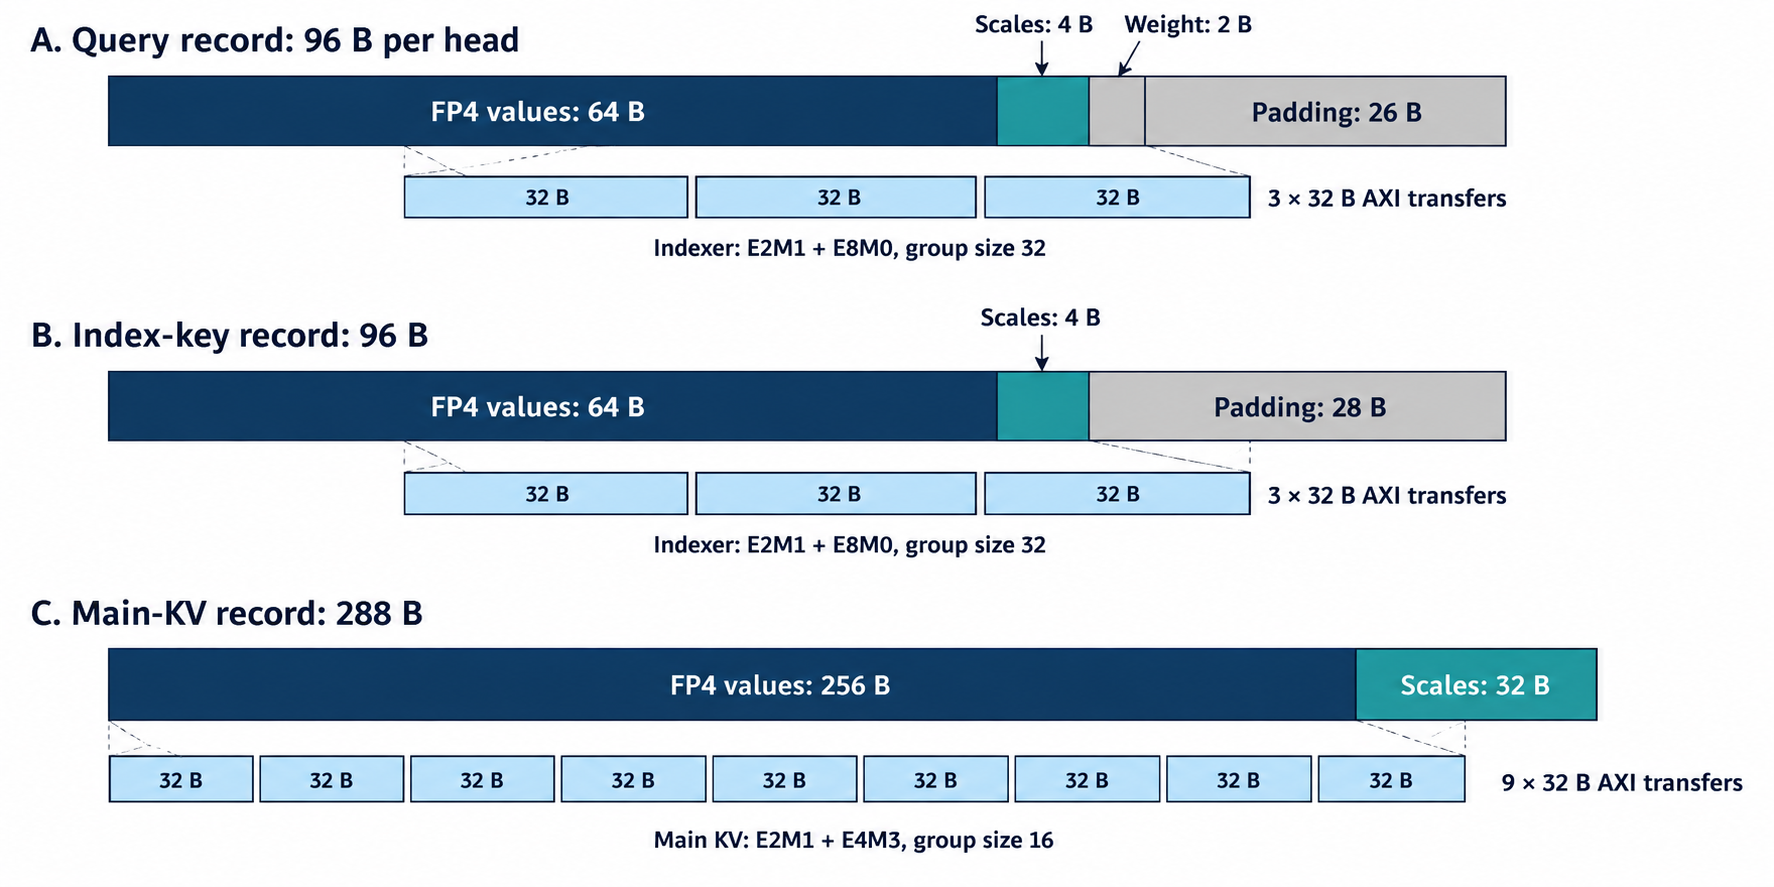
\includegraphics[width=.9\textwidth]{layout.png}
\caption{Physical record formats (schematic, not to scale). Index scales use E8M0/group32; main KV has an E2M1 payload with E4M3 scales/group16. Acceptance uses opaque deterministic 288-B patterns to verify gather, not trained main-KV activations or attention arithmetic. Padding and all AXI beats remain in the accounting.}
\label{fig:layout}
\end{figure*}

\section{Online Integration and Completion}
\subsection{RTL boundary and protocol adapter}
The original storage target produces whole-burst C++ FIFO objects rather than RTL AXI pins. A new dispatcher translates register requests into actual slave-channel handshakes and RTL DMA traffic back into requests for the same MemSimBackend. It does not calculate scores, maintain a private data image, or predict memory completion. Native mem\_sim accepts a request and later returns its bytes and completion event; those events drive the RTL response channels.

The RTL top has 64-bit addresses, 16-bit IDs, 256-bit data, and 32-bit WSTRB. The acceptance memory aperture is 1 MiB with a reserved 4-KiB MMIO window; buffer ranges must fit this configured aperture. Exclusive requests are rejected by the dispatcher. AW and W are buffered independently; response payloads hold through backpressure. The supported slave subset accepts naturally aligned single-beat accesses up to 32 B. Unsupported bursts return an error and are drained. The DMA emits one aligned 32-B INCR beat at a time. Internal response tags are distinct from the original processor-side IDs, avoiding aliasing when the DMA uses ID 1.

All Verilator evaluation occurs on the existing SystemC clock edges, using the same femtosecond time as gem5. No second SystemC kernel is linked. Standard traffic keeps its own queue and shares the online backend with DMA traffic. The first implementation has one outstanding DMA request, a deliberate throughput limitation.

\subsection{Execution modes and commit rule}
FULL scans the caller-provided valid key interval. REINDEX reads only the supplied candidate positions, checking uniqueness, ascending order, and bounds. REUSE requires a committed selection and matching context, epoch, key count, head count, K, Q address, and K address. It performs no Q/K reads or scoring; it still issues result writes and the requested KV gather. Software increments the epoch or invalidates the cache whenever source data change. This explicit protocol is not hardware coherence or an access-control mechanism.

Each result is a 32-B record containing index and FP32 score bits with zero padding. Selected packed main-KV records are read and copied to the gather output in index order. DONE is committed only after all output BRESPs succeed. A failing command may have partial writes, but its error status forbids their consumption as a complete result. A new command can recover from error. In-flight external reset recovery is outside the contract.

\begin{figure*}[t]
\centering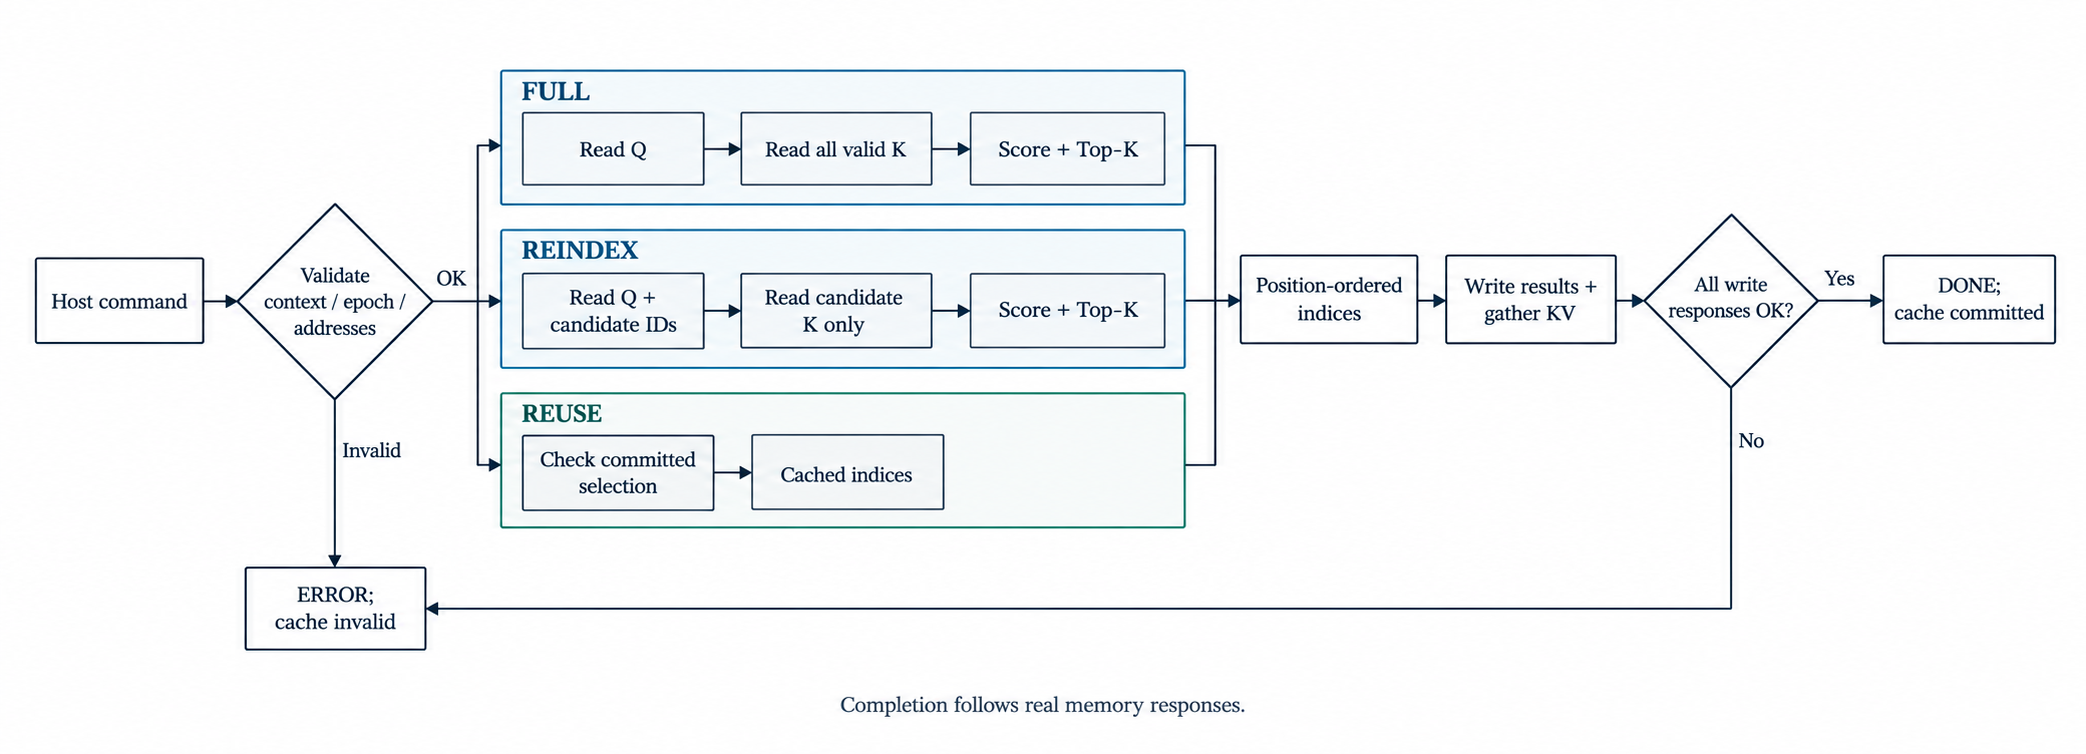
\includegraphics[width=.95\textwidth]{flow.png}
\caption{Command lifecycle. Candidate blocks are produced externally and expanded to valid indices. Reuse bypasses scoring, while every mode that produces output still waits for actual memory write responses before committing completion. The error/cache-invalidation path applies to an accepted START; an illegal doorbell is rejected without invalidating an earlier cache.}
\label{fig:flow}
\end{figure*}

\subsection{Traffic accounting}
Let $1\le C\le N$ be the valid candidate count; empty REINDEX lists are rejected. The result count is $R=\min(K,N)$ for FULL, $R=\min(K,C)$ for REINDEX, and the previously committed result count for REUSE. In particular, reuse after a short candidate list retains its smaller count. With $V$ a multiple-of-32 KV record size, the physical DMA beat counts are
\begin{align}
 B^\mathrm{full}_\mathrm{read}&=3H+3N+RV/32,\\
 B^\mathrm{reindex}_\mathrm{read}&=3H+3C+\lceil C/8\rceil+RV/32,\\
 B^\mathrm{reuse}_\mathrm{read}&=RV/32,\\
 B_\mathrm{write}&=R(1+V/32).
\end{align}
These counts exclude processor-side initial uploads, MMIO, result readback, and UCIe framing, which are separately present in the system traces. Reuse and hierarchical candidates are existing CSA2 mechanisms; their lower traffic is not presented as a new algorithmic discovery. A complete comparison must also include a compute-side resident index cache, rather than assume every competing method reloads all keys across UCIe.

\section{Validation Method and Results}
\subsection{Independent reference and pretrained weights}
Official source files and five layer-20 indexer tensors are locked to a specific revision. HTTP range requests retrieve exactly \TensorBytes{} tensor bytes rather than the complete checkpoint. They provide learned Q/K projections, normalization, and head weights. Gaussian intermediate activations are independently seeded and explicitly labeled synthetic. They are not hidden states extracted from text-driven full-model inference.

The oracle represents intermediate finite values as integer dyadics and independently performs IEEE FP32 rounding. It is cross-checked against \OraclePairCount{} NumPy finite input pairs for each of addition and multiplication and \RationalCaseCount{} exact-rational rounding-cell checks. The RTL's arithmetic helpers are checked on \FpCaseCount{} cases, including overflow and subnormal cases. The accepted core corpus has \CoreCaseCount{} cases, \CoreKeyCount{} successful key scores, and \CoreMacCount{} executed FP4 product terms. Error cases require the expected error and no selected output. Full H32/N640/K512 learned-weight-derived inputs and candidate-only inputs are included.

\begin{table}[t]
\centering\caption{Selected core cases. C denotes the submitted candidate count when only a subset of N positions is scanned. Cycles include the documented byte-load interface and test backpressure; these are not system latency measurements.}
\label{tab:core}
\small
\begin{tabular}{lrrrrl}\toprule
Case & H & N & K & Cycles & Check\\\midrule
Random full shape & 32 & 521 & 512 & 362,348 & PASS\\
Shuffled tied IDs & 4 & 35 & 9 & 5,669 & PASS\\
Signed head weights & 2 & 20 & 7 & 2,490 & PASS\\
Subnormal scores & 1 & 13 & 8 & 1,372 & PASS\\
Subset (C=22) & 4 & 64 & 12 & 3,758 & PASS\\
Weights: Top-512 & 32 & 640 & 512 & 444,514 & PASS\\
Weights: small full & 32 & 64 & 8 & 46,101 & PASS\\
Weights: C=16 & 32 & 64 & 8 & 13,250 & PASS\\
\bottomrule\end{tabular}
\end{table}


For the learned-weight N640 case, executing the two official score expressions on CPU in FP32 produces the same scores as the chosen ordered contract on this particular input. The BF16 expression has relative L2 difference \BfRelative{} and maximum absolute difference \BfAbsolute{}, with the same Top-512 set. This is one operator observation, not a universal equivalence or accuracy guarantee. For an all-zero N520 case, stable small-index selection and Torch's unspecified tie selection have a \TieDifference{}-element symmetric difference with equal tied scores. The artifact retains both results.

\subsection{AXI behavior and online evidence}
The wrapper test drives W-before-AW and AW-before-W transactions, randomized DMA acceptance/response delay, held slave responses, stale epochs, duplicate/out-of-range candidates, invalid formats, R/B failures, output/input overlap, and address wrap. It verifies each selected score and each gathered byte, and checks that stalled channel payloads remain stable. Its byte-addressed test memory is separate from the subsequent native-system evidence.

The original path passes 19 native tests, 7 CPU/tester cases, and 4 XPU cases. SparseGate then passes separate synthetic-input CPU, learned-weight-derived CPU, and three-source coexistence programs. The latter executes the original GPU/NPU work before gate commands; it demonstrates coexistence on the retained path, not concurrent gate contention.

Every gate run checks all returned score/index records and every gathered byte against the independent fixture. The small-case sequence exercises FULL, valid REUSE, REINDEX, stale-epoch rejection, and FULL recovery. The stale command has no accepted DMA traffic. Native AXI waves, UCIe Flits, backend events, and memory commands are cross-checked, with binary and source digests retained. Each command counter is independently checked against its RTL busy interval, and successful DONE is checked against the final DMA write response. A separate adapter/RTL test rejects unsupported exclusive accesses and verifies ordinary-access recovery.

The waveform checker also rejects three controlled corruptions of a recorded trace: an incremented cycle count, an incremented DMA-read count, and premature DONE at the final B handshake. These overlays leave the original simulation files unchanged.

\begin{figure*}[t]
\centering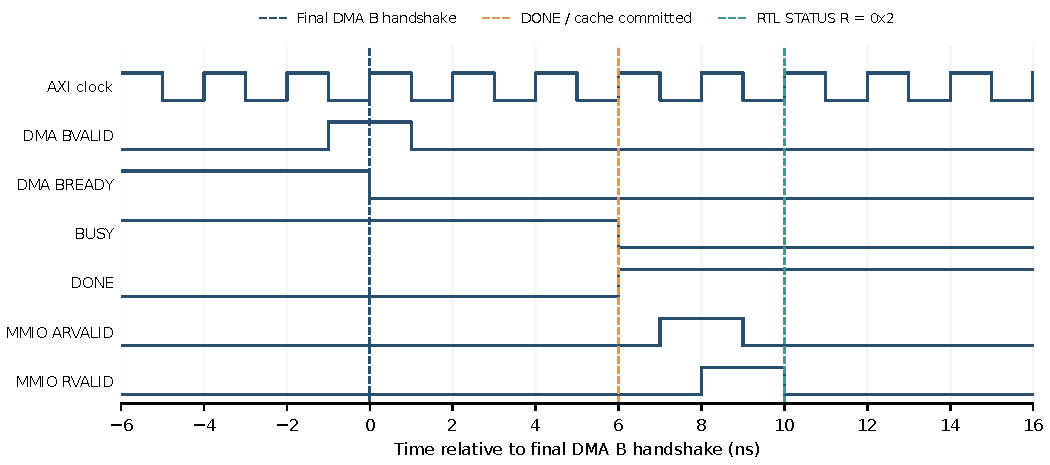
\includegraphics[width=.94\textwidth]{completion_wave.pdf}
\caption{Actual native RTL VCD samples around the first successful FULL completion in the H4/N16/K4 CPU program. Levels are recorded after model evaluation; handshakes sample values stable before the rising edge. DONE commits three AXI cycles after the final B handshake. The RTL STATUS response is independently correlated with its later delivery through the return protocol path. This is a simulator waveform, not a silicon capture.}
\label{fig:completion}
\end{figure*}
\begin{table}[t]
\centering\caption{Measured RTL command counters in the learned-weight-derived H32/N64/K8 program; REINDEX has 16 candidates. R/W are DMA beat counts, unchanged across the two memory periods. Each result gathers 288 B.}
\label{tab:modes}
\small
\begin{tabular}{lrrrrr}\toprule
Mode & Scores & R & W & $1\times$ cyc. & $4\times$ cyc.\\\midrule
FULL & 64 & 360 & 80 & 55,155 & 67,969\\
REUSE & 0 & 72 & 80 & 1,949 & 5,783\\
REINDEX & 16 & 218 & 80 & 18,788 & 26,359\\
\bottomrule\end{tabular}
\end{table}
The AXI simulation period is 2 ns. Command cycles count the RTL busy interval through the final write response; host-run time also includes the protocol and software interactions. All three successful commands return eight records on this input.

Increasing the online memory period from 0.25 to 1 ns preserves the guest binary, RTL, scores, and DMA counts. All successful command counters increase; complete host finish time increases by 181.530 $\mu$s. Polling traffic can change, so this is a memory-feedback experiment rather than a fixed-instruction speedup comparison.

A separate full-shape H32/N640/K512 guest executes FULL and then REUSE to distinct destinations. It verifies all 512 score/index records, their padding, and 147,456 gathered bytes per command. FULL takes 670,572 busy cycles with 6,624 read beats and 5,120 write beats; REUSE takes 115,776 cycles with 4,608/5,120 read/write beats. This extends full-shape selection evidence through the actual online path; the small-case REINDEX/error sequence is a separate test.

\begin{figure*}[t]
\centering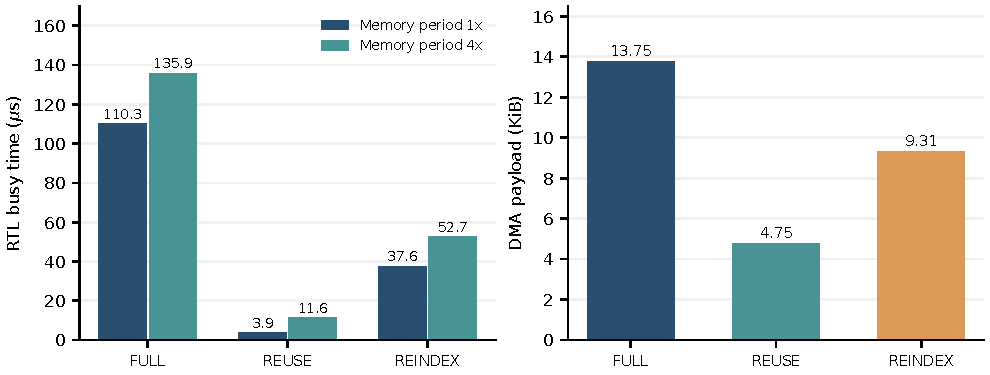
\includegraphics[width=.86\textwidth]{native_modes.pdf}
\caption{Measured H32/N64/K8 command latency with two online memory periods, and DMA payload (identical across periods). REUSE preserves an earlier selection; REINDEX evaluates a supplied subset. These different workloads are not interchangeable accuracy baselines. Payload includes result and gathered-KV writes, excluding host uploads, MMIO, readback, and link framing.}
\label{fig:native}
\end{figure*}


\subsection{Parallelism and implementation cost}
For a lane count $L$ dividing 32, the implemented sequential schedule has
\begin{equation}
 C_{\mathrm{arithmetic/key}}=H\left[4\left(\frac{32}{L}+2\right)+3\right].
\end{equation}
The two extra cycles per group perform conversion and FP32 addition; the remaining head costs include query-validity checking, weight multiplication, and head accumulation. At H32, this is 864/608/480 cycles for L8/L16/L32. Measured total latency additionally includes byte loading, heap work, and interface stalls. The figures below use counted cycles rather than ideal MAC-rate division.
\begin{figure}[t]
\centering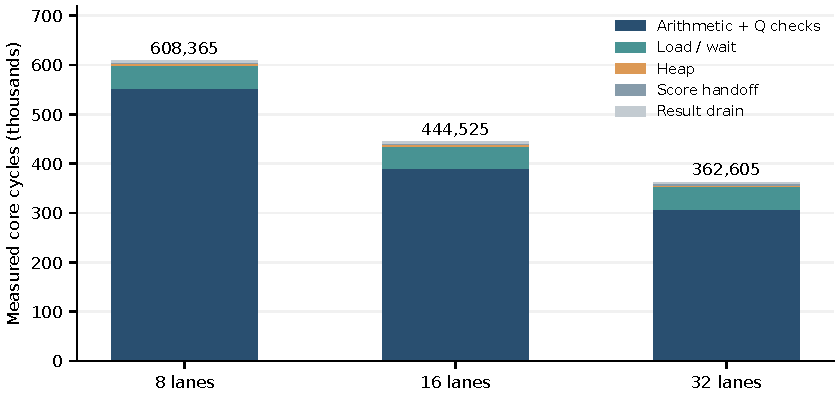
\includegraphics[width=\columnwidth]{lane_sweep.pdf}
\caption{Measured lane-count sensitivity for the same H32/N640/K512 learned-weight-derived input. All scores and selections match. This core-only test excludes wrapper positional sorting and native DMA/RAM waits; result-drain cycles reflect its testbench ready sequence. No clock or PPA equivalence across builds is assumed.}
\label{fig:lanes}
\end{figure}
The 8/16/32-lane implementations require 608,365, 444,525, and 362,605 cycles for the same input and identical handshake schedule. Each computes 2,621,440 product terms and selects the same 512 indices. Relative cycle improvements are 1.369$\times$ from 8 to 16 lanes and 1.226$\times$ from 16 to 32 lanes. More lanes shorten integer-product batches, while scale conversion and FP32 reduction remain serialized. Loading, selection and output costs remain visible; the result does not imply linear scaling or equal attainable frequency.

The 444,514-cycle Top-512 case in Table~\ref{tab:core} uses a different randomized backpressure sequence from this controlled lane sweep; the 444,525-cycle 16-lane result is therefore not an identical timing experiment.

\begin{table}[t]
\centering\caption{Native Design Compiler mapping of the 16-lane score/heap core in a TSMC 28-nm HPC+ standard-cell library. Arrays are flop-mapped. No layout, extracted interconnect, gate-level equivalence or physical signoff is claimed.}
\label{tab:synthesis}
\small
\begin{tabular}{lr}\toprule
Metric & Measured / configured\\\midrule
Library corner & TT 0.9V 25C\\
Target period (ns) & 2.000\\
Mapped cell area ($\mu$m$^2$) & 301,340.93\\
Leaf cells & 250,241\\
Sequential cells & 53,993\\
Setup slack (ns) & +0.000006\\
Hold slack (ns) & +0.005131\\
Design-rule violation entries & 0\\
Constraint coverage & PASS\\
\bottomrule\end{tabular}
\end{table}
The reported setup and hold checks meet the stated constraints in this mapped-core model. The reported setup margin is only 6 fs; this near-zero nominal margin is not evidence of a robust physical frequency. Design-rule entries count reported transition, capacitance, fanout, or other electrical-limit violations; an object appearing in multiple categories is counted in each. These checks are distinct from setup/hold and from layout DRC. The independent clock and I/O coverage checks pass, with the documented reset false-path exception. The report attributes 163,838.47 $\mu$m$^2$ to combinational cells and 137,502.45 $\mu$m$^2$ (45.6\%) to noncombinational cells. The latter includes control state as well as flop-mapped storage; it is not a measurement of Q/heap storage alone. For all 1,142 Liberty cells, the area exactly matches the same-name LEF width times height. The kit release compatibility is checked, and actual DC database areas match exactly. LEF SIZE dimensions use micrometers~\cite{lefdef}; this establishes cell-footprint area, not placed core or die area. The synthesis target excludes the AXI wrapper, DMA, processor models, and UCIe system. The clock is ideal; CTS and physical clock-network loading are not modeled. The tool uses a fanout estimate of 1,000 for the clock net reported with 53,993 loads. An independent saved-design readback checks mapping and timing reports; it is not an equivalence proof. The simulation clock is a test setting, not an established chip frequency.


\section{Discussion and Limits}
The evidence establishes reproducible operator arithmetic and live memory feedback, not full-model throughput, quality, energy, or a production-chip clock. The tested processor coexistence does not establish GPU/NPU contention during gate execution.

The byte-load interface and single-outstanding DMA serialize work. The positional sort is intentionally simple, and flop-mapped state carries a substantial area cost. These limitations identify concrete next steps: wider Q/K loading, double buffering, overlapped score/heap work, bounded multirequest DMA, and characterized SRAM binding. Each should be evaluated at the same numerical contract and resource constraints. Full-scan index arithmetic still costs $NHD$ scalar products; sparsity of the final attention does not remove that cost.

This design adopts the thesis's locality and reduction ideas while replacing its pooled-block arithmetic and fixed-size selection. Its contribution is the system-specific datapath and integration contract for an existing algorithm. Broader architectural comparisons require matched numerical contracts, workloads, and resource constraints.

\section{Artifact Availability}
Source, fixed submodule revisions, RTL tests, public evidence summaries, source hashes, and paper-generation code are available in the independent repository~\cite{artifact}. Original upstream main is unchanged. Model weights and proprietary library files are not redistributed; bounded download scripts and local synthesis entry points are provided. Conceptual figures were generated with the image-generation tool from preserved prompts and checked against the implementation. Measured plots and tables are generated from evidence JSON. The manuscript is an engineering research draft, not a peer-reviewed publication.

\bibliographystyle{IEEEtran}
\bibliography{references}
\end{document}
